%%%%%%%%%%%%%%%%%%%%%%%%%%%%%%%%%%%%%%%%%%%%%%%%%%%%%%%%%%%%%%%%%%%%%%%%%%%%%%%%%%%%%%%%%%
%%
%% Description:		This is an example presentation using the beamerthemedhbw
%%
%%					The beamerthemedhbw is based on jacksbeamertheme
%%					(https://github.com/JacknJo/jacksbeamertheme)
%%
%% Author:			Hannes Bartle																				
%% 					DHBW Ravensburg Campus Friedrichshafen		
%%					September 2016	
%% 
%% The beamerthemedhbw is free software: you can redistribute it and/or modify
%% it under the terms of the GNU General Public License as published by
%% the Free Software Foundation, either version 3 of the License, or
%% (at your option) any later version.
%% 
%% The beamerthemedhbw is distributed in the hope that it will be useful,
%% but WITHOUT ANY WARRANTY; without even the implied warranty of
%% MERCHANTABILITY or FITNESS FOR A PARTICULAR PURPOSE.  See the
%% GNU General Public License for more details.
%% 
%% You should have received a copy of the GNU General Public License
%% along with the beamerthemedhbw.  If not, see <http://www.gnu.org/licenses/>.
%% 
%% 
%%%%%%%%%%%%%%%%%%%%%%%%%%%%%%%%%%%%%%%%%%%%%%%%%%%%%%%%%%%%%%%%%%%%%%%%%%%%%%%%%%%%%%%%%%


\documentclass[	12pt, 				
				t,					
				aspectratio=169,
				%handout-PLACEHOLDER
				]{beamer}

\usepackage{dhbwstyle}

\title{Java GUI Grundlagen}

\begin{document}
	
	\begin{frame}[noframenumbering]
		\titlepage
	\end{frame}


	\begin{frame}{Inhalt}
		\tableofcontents
	\end{frame}
    
    \outlineFrame{Historie}
    \begin{frame}{Java GUI Anwendungen}{Die Historie}
    \begin{itemize}
        \item
        \item
        \item
        \item
        \item
    \end{itemize}
\end{frame}
    
    \outlineFrame{Grundlegender Aufbau}
    \begin{frame}{Swing}{Grundlegendes}
	\begin{itemize}
		\item AWT Komponenten erzeugen Komponenten über Betriebssystemaufrufe
		\item Dadurch Speicher nicht über Java verwaltet
		\item Swing erzeugt Komponenten über direkte Low-Level Calls
		\item Jede Komponente wird auf den Bildschirm gezeichnet
		\item Dadurch komplette Speicherverwaltung in Java
		\item Overhead führt ggf. zu Performanceverlust
		\item Aber mehr Kontrolle über die Features
	\end{itemize}
\end{frame}

\begin{frame}{Swing}{Konzepte}
	\begin{itemize}
		\item Swing nutzt das Entwurfstmuster des \textit{Kompositums}
		\item Kompositum beschreibt im Grunde eine Art Baumstruktur
		\item Objekte werden zu Gruppen zusammengefasst und Gruppen wiederum zu größeren Gruppen
		\item Dadurch kann eine einheitliche Behandlung von Objekten und Aggregaten erreicht werden
		\item Gemeinsame Eigenschaften von Objekt und Aggregat werden in einer Oberklasse isoliert
	\end{itemize}
\end{frame}

\begin{frame}{Beispiel für Kompositum}{Zusammengesetzte Grapfik-Objekte (Vgl. \cite{judt2017} S. 26}
	\includegraphics*[width=.8\textwidth]{graph/compositum_example}
	Gemeinsame Operationen: \texttt{zeichne()}, \texttt{verschiebe()}, \texttt{lösche()}, \texttt{skaliere()}
\end{frame}

\begin{frame}{Kompositum}{Beispielhaftes Klassendiagramm}
	\includegraphics*[width=.8\textwidth]{graph/compositum_cd}
\end{frame}

\begin{frame}{Kompositum}{Umsetzung in Swing}
	\begin{itemize}
		\item Die Klassenhierarchie stellt ein Kompositum dar
		\item Swing Objekte unterteilen sich hierbei in zwei Klassen:
		\begin{itemize}
			\item \texttt{Component}
			\item \texttt{Container}
		\end{itemize}
		\item \texttt{Container} fassen \texttt{Components} zusammen
		\item Jeder Container ist für die Anordnung seiner Komponenten zuständig
		\item Jeder \texttt{Container} ist auch immer eine \texttt{Component}
	\end{itemize}
\end{frame}

\begin{frame}{Klassendiagramm}{Der Swing Bibliothek}
	\includegraphics*[width=.8\textwidth]{graph/swing_cd}
\end{frame}

\begin{frame}{Swing Fenster}{JFrame Klasse}
	\begin{itemize}
		\item Basis eines Swing Fensters ist die \texttt{JFrame} Klasse
		\item Basiert auf der AWT Klasse \texttt{Frame}
		\item Lässt sich manipulieren z.B. in bezug auf
		\begin{itemize}
			\item Sichtbarkeit
			\item Größe und Position
			\item Operation beim schließen
		\end{itemize}
		\item Leeres Fenster wird erzeugt über den \texttt{JFrame()} Konstruktor
		%TODO: irgendwas irgendwas JFrame als basis
		%Referenz JFrame zu Frame?
	\end{itemize}
\end{frame}

\begin{frame}[fragile]{Swing Fenster}{Ganz simpel}
\lstset{style=java}
\begin{lstlisting}
public static void main(String[] args){
  JFrame window = new JFrame();
  window.setDefaultCloseOperation(WindowConstants.EXIT_ON_CLOSE);
  window.setVisible(true);
}
\end{lstlisting}
\end{frame}

\begin{frame}{JFrame}{Ändern der Größe des Fensters}
    \begin{itemize}
        \item Größe wird über \texttt{setSize()} verändert
        \item Hier gibt es zwei Überladungen:
        \begin{itemize}
            \item Als Parameter ein \texttt{Dimension} Objekt
            \item Zwei \texttt{int} Werte als Parameter
        \end{itemize}
    \end{itemize}
\end{frame}

\begin{frame}{Swing Fenster}{Weitere Eigenschaften}
    \begin{itemize}
        \item Bildet einen \textit{Top-Level-Container}
        \item Hinzufügen neuer Elemente über die \texttt{add()} Operation
        \item \texttt{JFrame} wird immer mit Titel und Menüleiste erzeugt
        \item Erscheinung des Frames kann geändert werden
        \begin{itemize}
            \item Man spricht in der Regel von "`Decorations"'
            \item Ändern der Form des Fensters (In begrenztem Rahmen)
            \item Wählen verschiedener Farbschema
            \item (Teil-)transparente Fenster
            \item usw
        \end{itemize}
    \end{itemize}
\end{frame}

\begin{frame}{Weitere Fenster in Swing}
    \begin{itemize}
        \item \texttt{JWindow} -- Fenster ohne Menüleiste
        \item \texttt{JDialog} -- Zum erstellen von (modalen) Dialogfeldern
    \end{itemize}
\end{frame}
    
    \outlineFrame{Grundlegende Komponenten}
    \begin{frame}{Komponenten}{Grundlegendes}
    \begin{itemize}
        \item Komponenten in Swing sind frei erweiterbar
        \item Swing Komponenten i.D.R. über Namensgebung von AWT Komponenten unterscheidbar
        \item Für viele Anwendungsfälle sind jedoch die Standardkomponenten schon ausreichen
        \item Neue Komponenten werden über \item{add()} Methode zu einem beliebigen Container hinzugefügt
        \item Komponenten können eine bevorzugte oder minimale Größe definieren
        \item Position wird i.d.R. automatisch bestimmt (Über den Layoutmanager)
    \end{itemize}
\end{frame}

\begin{frame}{Grundlegende Komponenten I}{Übersicht}
    \begin{itemize}[<+->]
        \item \texttt{JPanel} -- Einfacher Bereich ohne spezielle Besonderheiten. Ist ein \texttt{Container} und wird in der Regel genutzt um Elemente zu gruppieren und ggf. anzuordnen
        \item \texttt{JButton} -- Einfacher Button für den eine Funktion programmiert werden kann(Zum Beispiel das Starten einer Berechung)
        \item \texttt{JCheckBox} -- Auswahlbox für eine binäre Eingabe
        \item \texttt{JLabel} -- Simples Feld zum Anzeigen von Texten. Kann nicht durch den Nutzer bearbeitet werden
        \item \texttt{JTextField} -- Textfeld zum Anzeigen oder Bearbeiten von Texten (Einzelzeilen). Kann durch den Nutzer verändert werden
        \item \texttt{JSlider} -- Schieberegler
    \end{itemize}
\end{frame}

\begin{frame}{Grundlegende Komponenten II}{Übersicht}
	\begin{itemize}[<+->]
		\item \texttt{JRadioButton} -- Gibt die Möglichkeit zur Auswahl von einer Option aus mehreren gegebenen Möglichkeiten. Es kann pro Gruppe an Optionen immer nur genau eine gleichzeitig aktiviert sein. Um RadioButtons in Gruppen zusammenzufassen, ist die Nutzung eines \texttt{ButtonGroup} Objects notwendig
        \item \texttt{JComboBox} -- Element, das die Auswahl eines Eintrags aus einer Liste erlaubt oder auch einen eigenen Eintrag ermöglicht
        \item \texttt{JEditorPane} -- Ermöglicht die Eingabe von mehrzeiligen Texten
	\end{itemize}
\end{frame}
	
    \outlineFrame{Layout Manager}
    \begin{frame}{GUI Layout}{Anordnen von Elementen}
    \begin{itemize}
        \item Bei Nutzen von \texttt{add()} werden Komponenten automatisch platziert
        \item Dies geschieht durch den \textit{Layout Manager}
        \item Manager werden pro Container definiert
        \item Je nach Layout sind ggf. feste "`Slots"' im Container vorhanden
        \item Um Komponente an bestimmter Position zu platzieren wird Überladung von \texttt{add()} verwendet:
        \begin{itemize}
            \item \texttt{add(Component comp, Object constraint)}
            \item \texttt{constraint} definiert Position im Container
        \end{itemize}
    \end{itemize}
\end{frame}

\begin{frame}{GUI Layout}{Größe von Komponenten}
    \begin{itemize}
        \item Komponenten können absolute, minimale, maximale und bevorzugte Größe definieren
        \begin{itemize}
            \item \texttt{setSize(int height, int width)}
            \item \texttt{setMinimumSize(Dimension d)}
            \item \texttt{setMaximumSize(Dimension d)}
            \item \texttt{setPreferredSize(Dimension d)}
        \end{itemize}
        \item Layout Manager \textit{versucht} diese zu beachten
        \item \textit{Müssen} dies jedoch nicht
        \item Insbesondere absolute Größen sind meist gegen das Prinzip von Layout Managern
    \end{itemize}
\end{frame}

\begin{frame}{GUI Layout}{Layout Manager}
    \begin{itemize}
        \item Vorteil von Layout Managern:
        \begin{itemize}
            \item Relative Positionierung von Komponenten kann definiert werden
            \item Vereinfachen erstellen von GUIs
            \item Größe und Position von Komponenten werden automatisch angepasst (Zum Beispiel bei Ändern der Fenstergröße)
        \end{itemize}
    \end{itemize}
\end{frame}

\begin{frame}{BorderLayout}{Grundlegendes (Vgl. \cite{orac:borderlayout})}
    \begin{itemize}
        \item Teil den Container in fünf Bereiche
        \item Diese sind über Konstanten in der \texttt{BorderLayout} Klasse definiert:
        \begin{itemize}
            \item \texttt{PAGE\_START} -- Oberer Bereich (Kopfzeile)
            \item \texttt{PAGE\_END} -- Unterer Bereich (Fußzeile)
            \item \texttt{LINE\_START} -- Linker Bereich zwischen Kopf und Fuß
            \item \texttt{LINE\_END} -- Rechter Bereich zwischen Kopf und Fuß
            \item \texttt{CENTER} -- Mittlerer (Haupt-)bereich
        \end{itemize}
        \item Beispiel: Hinzufügen im \texttt{PAGE\_START} Bereich:
        \begin{itemize}
            \item \texttt{add(button, BorderLayout.PAGE\_START)}
        \end{itemize}        
    \end{itemize}
\end{frame}

\begin{frame}{BorderLayout}{Weitere Eigenschaften (Vgl. \cite{orac:borderlayout})}
    \begin{itemize}
        \item Fokus liegt auf den \texttt{CENTER} Bereich
        \item Dieser nutzt maximal verfügbaren Platz
        \item Alle anderen Bereiche nutzen nur den benötigten Platz
        \item Nicht alle Bereiche müssen genutzt werden
        \item \texttt{PAGE\_START} und \texttt{PAGE\_END} nutzen (sofern vorhanden) immer die volle Breite
        \item Freiräume zwischen Bereichen lassen sich definieren:
        \begin{itemize}
            \item \texttt{setHGap(int)}
            \item \texttt{setVGap(int)}
        \end{itemize}
        \item Standard-Layoutmanager von \texttt{JFrame}
    \end{itemize}
\end{frame}

\begin{frame}{BorderLayout}{Aufgabe}
    \begin{alertblock}{BorderLayout Demo}
    Implementiert eine simple Fensteranwendung, um das Verhalten des \texttt{BorderLayout} kennen zu lernen. Platziert dazu zunächst jeweils einen \texttt{JButton} in
    jedem Bereich. 
    
    Untersucht, wie sich die Größe und Anordnung der Buttons ändert, wenn ihr eine Größe für die Buttons definiert oder wenn ihr einzelne Bereiche im Layout ungenutzt lasst.
    \end{alertblock}
\end{frame}

\begin{frame}{BoxLayout}{Grundlegendes(Vgl. \cite{orac:boxlayout})}
    \begin{itemize}
        \item Ordnet Komponenten entweder vertikal oder horizontal angeordnet
        \item Dafür zwei Konstanten in der \texttt{BoxLayout} Klasse
        \begin{itemize}
            \item \texttt{PAGE\_AXIS} -- Vertikale Anordnung (Als eine "`Spalte"')
            \item \texttt{LINE\_AXIS} -- Horizontale Anordnung (Als eine "`Zeile"')
        \end{itemize}
        \item Komponenten werden dann gemäß \texttt{ComponentAlignment} platziert (Bspw. Linksbündig/Zentriert/Rechtsbündig)
        \item Definierte maximale Größe von Komponenten wird im \texttt{BoxLayout} \textit{immer} respektiert
    \end{itemize}
\end{frame}

\begin{frame}[fragile]{BoxLayout}{Aufgabe}
Entwerft eine Beispielandwendung, in der mehrere Buttons in einem Frame mit dem \texttt{BoxLayout} als Layout Manager. Nutzt folgende Basis um den Layout Manager im \texttt{JFrame()} anzupassen:

\lstset{style=java}
\begin{lstlisting}
JFrame frame = new JFrame();
frame.setSize(300,600);
frame.setLayout(new BoxLayout(window, BoxLayout.PAGE_AXIS));

/*Buttons hinzufügen*/

frame.setVisible(true);
\end{lstlisting}

Experimentiert, was passiert, wenn ihr die Orientierung der einzelnen Komponenten anpasst.
\end{frame}

\begin{frame}{FlowLayout}{(Vgl. \cite{orac:flowlayout})}
    \begin{itemize}
        \item Ist das Standard-Layout von \texttt{JPanel}
        \item Komponenten werden in einer Reihe nebeneinander platziert
        \item Hierbei wird die bevorzugte Größe der Komponenten berücksichtigt
        \item Ist in einer Reihe nicht genug Platz verbleibend für die neue Komponente, so wird eine neue Reihe eingefügt
        \item Positionierung der Reihen kann definiert werden:
        \begin{itemize}
            \item \texttt{BoxLayout.LEFT} -- Linksbündig
            \item \texttt{BoxLayout.RIGHT} -- Rechtsbündig
            \item \texttt{BoxLayout.CENTER} -- Zentriert
            \item \texttt{BoxLayout.LEADING} -- Bündig mit dem Beginn der Container-Orientierung (zB. Links bei Links-nach-Rechts Orientierung)
            \item \texttt{BoxLayout.TRAILING} -- Bündig mit dem Ende der Container-Orientierung (zB. Links bei Rechts-nach-Links Orientierung)
        \end{itemize}
    \end{itemize}
\end{frame}

\begin{frame}{FlowLayout}{Aufgabe}
\begin{alertblock}{}
Entwerft eine simple Fensteranwendung, die über das Hinzufügen mehrerer Buttons mit verschiedener Größe die Funktionsweise des \texttt{FlowLayouts} demonstriert. Ändert hierzu
entweder den LayoutManager des erzeugten \texttt{JFrame} Objekts(Siehe Aufgaben zum BoxLayout) oder fügt ein \texttt{JPanel} hinzu, dem ihr anschließend die Buttons hinzufügt.

Experimentiert mit dem Verhalten des FlowLayouts bei ändern der Fenstergröße.
\end{alertblock}
\end{frame}

\begin{frame}{GridLayout}{Grundlegendes (Vgl. \cite{orac:gridlayout})}
    \begin{itemize}
        \item Rastert den Container in Zeilen und Spalten
        \item Jede "`Zelle"' ist gleichgroß
        \item Komponenten in einer Zelle nehmen die gesamte Zelle ein
        \item Komponenten werden automatisch in die "`nächste"' Zelle hinzugefügt
        \item Initialisierung:
        \begin{itemize}
            \item \texttt{GridLayout()} -- Initialisiert den Container mit einem 1x1 Grid
            \item \texttt{GridLayout(int rows, int cols)} -- Initialisiert das Grid mit der definierten Anzahl an Zeilen und Spalten
        \end{itemize}
        \item Zeilen \textit{oder} Spalten können auf $0$ gesetzt werden $\rightarrow$ Heißt, dass die Anzahl der Zeilen/Spalten dynamisch aus Anzahl der Komponenten ermittelt wird
    \end{itemize}
\end{frame}

\begin{frame}{GridLayout}{Aufgabe}
\begin{alertblock}{}
Entwerft eine Simple Fensteranwendung in der ihr mehrere Komponenten mit dem GridLayout anordnet. Um den Layout Manager zu ändern geht vor wie im Beispielcode zur BoxLayout Aufgabe.

Untersucht, wie sich Anordnung der Komponenten verhält, wenn ihr die Anzahl der Zeilen oder Spalten mit $0$ definiert.
\end{alertblock}
\end{frame}

\begin{frame}{GridBagLayout}{Grundlegendes (Vgl. \cite{orac:gridbaglayout})}
    \begin{itemize}
        \item Ähnlich zum \texttt{GridLayout}
        \item Jedoch flexibler in der Positionierung
        \item Dadurch aber auch komplexer in der Anwendung
        \item Komponenten können in beliebigen Zellen platziert werden
        \item Komponenten können mehrere Zellen einnehmen
        \item Relative Positionierung von Komponenten in den Zellen möglich
    \end{itemize}
\end{frame}

\begin{frame}{GridBagLayout}{Visualisiert}
    \begin{onlyenv}<1|handout:0>
    \begin{figure}
        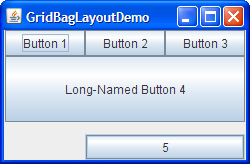
\includegraphics[height=5cm]{graph/gridbag}
        \caption*{\cite{orac:gridbaglayout}}
    \end{figure}
    \end{onlyenv}
    \begin{onlyenv}<2->
    \begin{figure}
        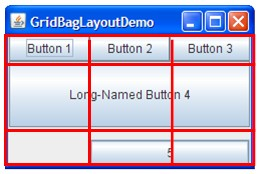
\includegraphics[height=5cm]{graph/gridbagline}
        \caption*{\cite{orac:gridbaglayout}}
    \end{figure}
    \end{onlyenv}
\end{frame}

\begin{frame}{GridBagLayout}{Constraints (Vgl. \cite{orac:gridbaglayout})}
    \begin{itemize}
        \item Platzierung der Komponenten im GridBag wird über \texttt{GridBagConstraints} Objekt definiert
        \item Diese müssen beim hinzufügen von Komponenten mit übergeben werden:
        \begin{itemize}
            \item \texttt{add(Component,GridBagConstraints)}
        \end{itemize}
        \item Für die Constraints lassen sich definieren:
        \item \textbf{\texttt{gridx, gridy}} -- Zeile und Spalte der hinzuzufügenden Komponente. Kann auch als relativ zur zuletzt hinzugefügten Komponente definiert werden
        \item \textbf{\texttt{gridwidth, gridheight}} -- definiert, wie viele Zeilen bzw. Spalten die Komponente einnehmen soll
    \end{itemize}
\end{frame}

\begin{frame}{GridBagLayout}{Constraints (Vgl. \cite{orac:gridbaglayout})}
    \begin{itemize}
        \item \textbf{\texttt{fill}} -- Definiert inwiefern die Komponente den verfügbaren Platz nutzen soll. Kann genutzt werden, um Komponenten horizontal bzw. vertikal auf die Größe der Zelle zu skalieren
        \item \textbf{\texttt{ipadx, ipady, insets}} -- Kann genutzt werden um padding der Komponente zum Rand zu definieren 
        \item \textbf{\texttt{anchor}} -- Definiert die Referenzposition in der Zelle (z.B. links unten, rechts oben etc.)
        \item \textbf{\texttt{weightx, weighty}} -- Wird genutzt um zu bestimmen, wie der gesamt verfügbare Platz auf die einzelnen Zeilen/Spalten verteilt wird. Insbesondere wichtig, wenn die Fenstergröße verändert wird.
    \end{itemize}
\end{frame}

\begin{frame}{GridBagLayout}{Aufgabe}
Experimentiert (wenn ihr wollt) mit dem GridBagLayout und den entsprechenden Constraints. Zur Orientierung könnt die Oracle Tutorial Seite nutzen(Siehe \cite{orac:gridbaglayout})
\end{frame}

\begin{frame}{Layout Manager}{Kombinieren von Layout Managern}
    \begin{itemize}
        \item Komplexe GUIs erfordern nicht zwingend einen komplexen LayoutManager
        \item Da jeder Container Layout Manager selbst definiert können diese kombiniert werden
        \item Heißt: Ein Container wird einem übergeordneten Layout hinzugefügt, verwendet aber für seine eigenen Komponenten einen anderen Manager
        \item Als Basis-Container wird meist ein \texttt{JPanel} verwendet
    \end{itemize}
\end{frame}

\begin{frame}{Layout Manager}{Aufgabe}
\begin{alertblock}{}
Entwerft eine simple GUI Anwendung mit einem BorderLayout. Platziert beliebige Komponenten in den äußeren Bereichen. Platziert im Center Bereich ein \texttt{JPanel}, in dem Komponenten im \texttt{BoxLayout} angeordnet sind.
\end{alertblock}
\end{frame}

\begin{frame}{GUI-Builder}{}
    \begin{itemize}
        \item Alternativ zum "`ausprogrammieren"' der GUI können auch GUI-Builder verwendet werden
        \item Hier werden die Komponenten in einer grafischen Oberfläche platziert
        \item Struktur wird dann meist in XML Format (o.Ä.) übersetzt
        \item Spezieller Layout Manager übernimmt Übersetzung in Code
        \item In IntelliJ integriert
        \item Für Eclipse als Plug-In verfügbar
    \end{itemize}
\end{frame}
    
    \outlineFrame{Eigene Komponenten}
    \begin{frame}{Eigene Fenster}{Erstellen von Fenstern}
    \begin{itemize}
        \item Unsere bisherigen Fenster haben wir uns in der \texttt{main} zusammengebastelt
        \item Dies ist in der Regel unpraktikabel
        \item Code ist nicht wiederverwendbar
        \item Und ggf. schwierig wartbar
        \item Angestrebt wird eine Trennung von Darstellung und Logik und Daten
        \item Daher: Kapselung von GUI in eigene Klasse
        \begin{itemize}
            \item Diese erbt von \texttt{JFrame}
            \item Fenster wird im Konstruktor "`zusammengebaut"'
            \item Hinzufügen aller Komponenten, Layouten von diesen, setzen von Attributen wie Größe etc.
            \item In der Main Klasse wird dann lediglich ein Objekt von unserer neuen \texttt{JFrame} Unterklasse erzeugt
        \end{itemize}
    \end{itemize}
\end{frame}

\begin{frame}{Eigene Komponenten}{Grundlegendes}
    \begin{itemize}
        \item Erben vom \texttt{JComponent} Typ
        \item Lassen sich vielseitig konfigurieren z.B. in:
        \begin{itemize}
            \item Aussehen
            \item Verhalten
        \end{itemize}
        \item Nützlich kann es zum Beispiel sein die \texttt{getXxxSize} Methode zu überschreiben, wenn eine Komponente immer eine bestimmte Größe haben soll
        \item Fokus heute: Zeichnen von eigenen Komponenten
    \end{itemize}
\end{frame}

\begin{frame}{Zeichnen von Komponenten}{Schritte im \texttt{paint()} Prozess}
    \begin{itemize}
        \item Jede Komponente besitzt eine \texttt{paint()} Methode
        \item In dieser wird das Aussehen der Komponente auf den Bildschirm gezeichnet
        \item \texttt{paint()} ruft drei Methoden (in dieser Reihenfolge) auf:
        \begin{itemize}
            \item \texttt{paintComponent(Graphics g)}
            \item \texttt{paintBorder(Graphics g)}
            \item \texttt{paintChildren(Graphics g)}
        \end{itemize}
        \item In der Regel reicht es aus \texttt{paintComponent()} zu überschreiben
        \item Wir rufen \texttt{paint()} bzw. \texttt{paintComponent()} \textbf{nie} direkt auf
    \end{itemize}
\end{frame}

\begin{frame}{Zeichnen von Komponenten}{Die \texttt{paint()} Methode}
    \begin{itemize}
        \item \texttt{paint()} Wird durch das System automatisch aufgerufen bei zB.:
        \begin{itemize}
            \item Verschieben des Fensters/Von Komponenten
            \item Ändern der Fenstergröße
            \item Minimieren/Maximieren
        \end{itemize}
        \item Wenn programmatisch neu gezeichnet werden muss (Zum beispiel weil sich Daten geändert haben) wird die \texttt{repaint()} Methode aufgerufen
        \item \texttt{repaint()} akzeptiert Argumente, sodass nur ein bestimmter Bereich neu gezeichnet wird
    \end{itemize}
\end{frame}

\begin{frame}{Das \texttt{Graphics} Objekt}{Zeichnen von Komponenten}
    \begin{itemize}
        \item Den \texttt{paintXXX()} Methoden wird ein Objekt vom Typ \textit{Graphic} übergeben
        \item Dieses fasst verschiedene Aspekte zum Zeichnen zusammen:
        \begin{itemize}
            \item Aktuelle Komponente auf die gezeichnet wird
            \item Die Aktuelle Farbe
            \item Die aktuelle Font
            \item Weitere Aspekte die für die aktuelle Betrachtung nicht von Relevanz sind
        \end{itemize}
        \item Die Graphics Klasse bietet einige Funktionen zum Zeichnen von primitiven Formen an
    \end{itemize}
\end{frame}

\begin{frame}{Das \texttt{Graphics} Objekt}{Zeichenoperationen}
    \begin{itemize}
        \item \texttt{drawString} -- Zeichnet einen gegebenen String an der angegebenen Position (Mehrere Überladungen)
        \item \texttt{drawImage} -- Zeichnet ein Bild an einer bestimmten Stelle (Mehrere Überladungen)
        \item \texttt{drawArc} -- Zeichnet einen Ellipsenbogen
        \item \texttt{drawLine} -- Zeichnet eine Linie zwischen zwei Punkten
        \item \texttt{drawOval} -- Zeichnet ein Oval
        \item \texttt{drawRect} -- Zeichnet ein Rechteck
        \item \texttt{drawRoundRect} -- Zeichnet ein abgerundetes Rechteck
    \end{itemize}
\end{frame}

\begin{frame}{Zeichnen von Komponenten}{Weitere nützliche Operationen}
    \begin{itemize}
        \item Über \texttt{getWidth()} bzw. \texttt{getHeight()} kann die aktuelle Größe der Komponenten bestimmt werden
        \item Für viele der \texttt{drawXXX} Methoden existieren analoge \texttt{fillXXX} Methoden
        \item Aktuelle Zeichenfarbe lässt sich ändern über \texttt{setColor}
        \item Analog lässt sich \texttt{setFont} verwenden um die Schriftart zu ändern
    \end{itemize}
\end{frame}

\begin{frame}{Hinweise}{Beim Entwerfen von View-Komponenten}
    \begin{itemize}
        \item Die Komponenten sollten nur für die Darstellung verantwortlich sein
        \item In ihnen werden in der Regel keine Applikationsdaten gespeichert
        \item Auch die Logik ist in der Regel entkoppelt von der Darstellung
        \item Man spricht hierbei auch vom \textit{Model-View-Controller (MVC)} Konzept:
        \begin{itemize}
            \item Model -- Tatsächlich verwendetes Datenmodell. Speichert die Applikationsdaten (Datenschicht)
            \item View -- Anzeigen/rendern von Daten. Dient lediglich zur Darstellung (Präsentationsschicht)
            \item Controller -- Realisiert die Steuerung in Interaktion des Nutzers. Bildet in der Regel die Kopplung zwischen Model und View (Interaktionsschicht)
        \end{itemize}
    \end{itemize}
\end{frame}
    
    \outlineFrame{Aufgaben}
    \begin{frame}{Aufgaben 1}{KeyValue-Pair}
    Entwickelt eine \texttt{Pair}-Klasse, die zwei Instanzvariablen (\texttt{Key} und \texttt{Value}) speichert. Definiert die Instanzvariablen über die Nutzung von Generics.
    Implementiert einen Konstruktor, mit dem ein \texttt{KeyValue}-Objekt erzeugt wird und die beiden Instanzvariablen initialisiert. Baut Methoden ein, um die Werte unabhängig voneinander abzurufen und zu setzen.
\end{frame}

\begin{frame}[allowframebreaks]{Aufgabe 2}{Array-Wrapper Klasse}
    Entwickelt eine Wrapper Klasse für Arrays. Die Klasse soll ein Array eines generischen Typs speichern.

    Außerdem sollte die Klasse folgende Funktionen implementieren:
    \begin{enumerate}
        \item Konstruktor dem die initialen Daten für das Array übergeben werden
        \item \texttt{printData} - Gibt den Inhalt des Arrays auf der Kommandozeile aus
        \item \texttt{getData}/\texttt{setData} - Setzen das gespeicherte Array bzw. geben dieses zurück
        \item \texttt{getElement}/\texttt{setElement} - Setzen ein bestimmtes Element (über Angabe des Indizes) bzw. geben dieses zurück
        \item \texttt{contains} - Überprüft ob ein bestimmtes Element im Array vorhanden ist
        \item \texttt{countOccurences} - Zählt die Vorkommen eines bestimmten Elements im Array
        \item \texttt{invertArray} - Kehrt die Reihenfolge der Daten im gespeicherten Array um
    \end{enumerate}
\end{frame}

\begin{frame}{Aufgabe 3}{Aufgabe 3: Erweiterung der Wrapper-Klasse für \texttt{Number}}
    Erweitert die in 2. entwickelte Klasse so, dass das gespeicherte Array vom Typ \texttt{Number} (oder einer der Subtypen) sein muss.

    Implementiert zusätzlich folgende Methoden:
    \begin{enumerate}
        \item \texttt{getSum} - Ermittelt die Summe aller Elemente im Array
        \item \texttt{getProduct} - Ermittelt das Produkt aller Elemente im Array
        \item \texttt{getDifference} - Ermittelt die Differenz aller Elemente im Array
        \item \texttt{getMin}/\texttt{getMax} - Ermittelt Mini- bzw. Maximum aller Elemente
        \item \texttt{getAverage} - Bestimmt das arithmetische Mittel
    \end{enumerate}

    Hinweis: Nutzt hierfür die \texttt{doubleValue()} Methode der \texttt{Number} Klasse
\end{frame}

\begin{frame}[allowframebreaks]{Aufgabe 4}{Erweiterung der Wrapper Klasse für \texttt{Comparable}}

    Erweitert die in 2. entwickelte Klasse so, dass der Typ des gespeicherten Arrays das \texttt{Comparable} Interface implementieren muss.

    Implementiert zusätzlich folgende Methoden:
    \begin{enumerate}
        \item \texttt{getMin}/\texttt{getMax} - Ermittelt Mini- bzw. Maximum aller Elemente
        \item \texttt{allSmaller} - Überprüft, ob alle Werte im Array kleiner als ein gegebener Wert sind
        \item \texttt{allGreater} - Überprüft, ob alle Werte im Array größer als ein gegebener Wert sind
        \item \texttt{allInRange} - Überprüft, ob alle Werte im Array zwischen zwei gegebenen Werten liegen
        \item \texttt{allOutOfRange} - Überprüft, ob alle Werte im Array außerhalb von zwei gegebenen Werten liegen
        \item \texttt{clamp} - Es wird eine untere und eine obere Grenze übergeben. Alle Werte im Array die kleiner als die untere Grenze sind, werden auf diesen Wert gesetzt. Analog geschieht das mit der oberen Grenze
    \end{enumerate}

    Hinweis: Nutzt hierfür die \texttt{compareTo(T)} Methode des \texttt{Comparable<T>} Interfaces
\end{frame}

\begin{frame}[allowframebreaks]{Aufgabe 5}{Wildcards}
Entwickelt eine Klasse, die verschiedene statische Methoden für Listenoperationen zur Verfügung stellt. 

Nutzt hierbei zur Umsetzung Wildcards.
Implementiert mindestens die folgenden Funktionen:

\begin{enumerate}
    \item Eine Methode, die alle Elemente einer übergebenen Liste ausgibt (Ähnlich wie \texttt{printData()} aus Aufgabe 2)
    \item Eine Methode, die für eine beliebige Liste vom Typ \texttt{Number} die Summe berechnet
    \item Eine Methode, die zwei Listen vom Typ \texttt{Number}(Oder der Unterklassen) zu einer einzigen kombiniert. (Hinweis: sowohl die beiden Eingabelisten, 
    als auch die Ausgabeliste sollen als Parameter übergeben werden)
    \item Eine Methode, die für zwei Listen eines beliebigen \texttt{Number} Typs die Elementweise Summe berechnet und diese in einer neuen Liste speichert.
\end{enumerate}
\end{frame}
    
    \printbibliographyframe
    
	\section*{Kontakt}
	\begin{frame}{Kontakt}{}
	\begin{itemize}
		\item E-Mail: \href{mailto:lukas.abelt@airbus.com}{lukas.abelt@airbus.com}
		\item GitHub: \url{https://www.github.com/LuAbelt}
		\item GitLab: \url{https://www.gitlab.com/LuAbelt}
		\item Telefon(Firma): 07545 - 8 8895
		\item Telegram: LuAbelt
	\end{itemize}
\end{frame}
	

\end{document}